%! TeX program = xelatex
\documentclass{article}
\usepackage{amsmath}
\usepackage{amssymb}
\usepackage{fontspec}
\usepackage{graphicx}
\usepackage{tikz}
\usepackage[normalem]{ulem}
\usepackage[margin=0.75in]{geometry}

\graphicspath{{../../../}}

\setmainfont{Noto Serif CJK KR}
\title{2. 집합의 연산 step C 풀이}
\author{
    
\includegraphics[scale=0.25]{logo}
}
\date{}

\begin{document}
\maketitle

\paragraph{1번}
$\mathrm{P}(A)$는 $A$의 모든 부분집합을 원소로 갖는 집합임을 알 수 있다. 간단하게 $\mathrm{P}(A)$와 $\mathrm{P}(B)$를 계산하면 다음과 같다.

\[
    \mathrm{P}(A) = \{\varnothing, \{0\} \}, \mathrm{P}(B) = \{\varnothing, \{0\}, \{1\}, \{0, 1\}\}
\]

따라서 보기 중 성립하는 것은 \underline{2}밖에 없다.

\paragraph{2번}
이 문제는 그래프를 통해 해결 가능하다. 각각의 집합 $A$, $B$, $C$를 나타내면 다음과 같다.

\begin{center}
    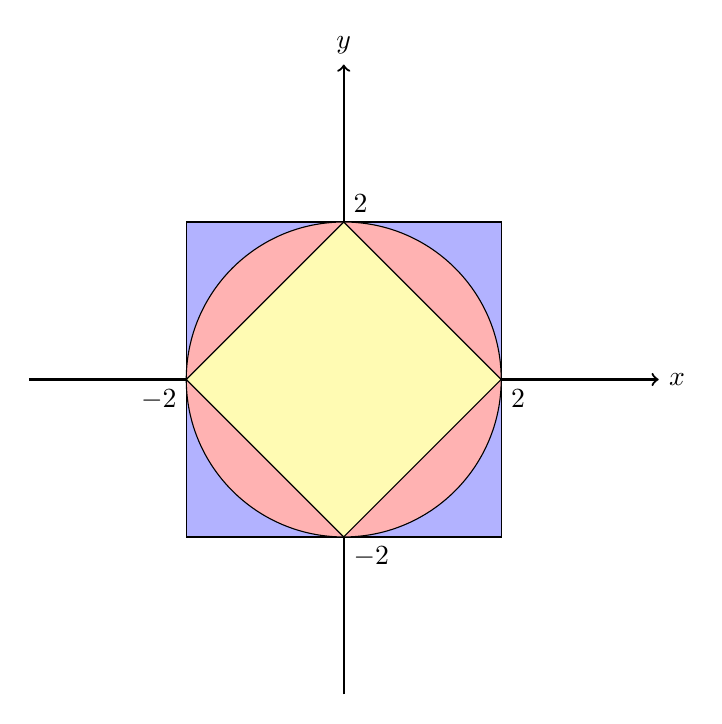
\begin{tikzpicture}
        \draw[thick,->] (-4, 0) -- (4, 0) node[anchor=west] {$x$};
        \draw[thick,->] (0, -4) -- (0, 4) node[anchor=south] {$y$};
        \filldraw[color=black, fill=blue!30] (-2,-2) rectangle (2,2);
        \filldraw[color=black, fill=red!30] (0, 0) circle (2);
        \filldraw[color=black, fill=yellow!30] (0, 2) -- (2, 0) -- (0, -2) -- (-2, 0) -- cycle;
        \draw[shift={(2, 0)}] node[below right] {$2$};
        \draw[shift={(-2, 0)}] node[below left] {$-2$};
        \draw[shift={(0, 2)}] node[above right] {$2$};
        \draw[shift={(0, -2)}] node[below right] {$-2$};
    \end{tikzpicture}
\end{center}

이 그림에서 파랑, 빨강, 노랑 도형은 각각 집합 $A$, $B$, $C$를 나타낸다. 즉, $C \subset B \subset A$를 알 수 있고, 보기에서 맞는 것을 고르면 \underline{2}이다.

\paragraph{3번}
문제에 주어졌듯, $A_n$은 다음과 같다. (편의상 $\mathbb{N}$을 자연수의 집합이라고 하자.)

\[
    A_n = \{x \mid 2n \le x < 8n + 6, x, n \in \mathbb{N}\}
\]

$n \rightarrow n + 1$일 때, 식은 다음과 같다.

\[
    A_{n + 1} = \{x \mid 2n + 2 \le x < 8n + 14, x, n \in \mathbb{N}\}
\]

이때, $A_n \cap A_{n + 1}$은 다음과 같을 것이다.

\[
    A_n \cap A_{n + 1} = \{x \mid 2n + 2 \le x < 8n + 6, x, n \in \mathbb{N}\}
\]

좀 더 일반화시키면, $A_{n + k}$는 다음과 같을 것이고,

\[
    A_{n + k} = \{x \mid 2(n + k) \le x < 8(n + k) + 6, x, n, k \in \mathbb{N}\}
\]

이때, $A_n \cap A_{n + k}$는

\[
    A_n \cap A_{n + k} = \{x \mid 2(n + k) \le x < 8n + 6, x, n, k \in \mathbb{N}\}
\]

그냥 넘어가지 말고 위의 식들과 비교하며 패턴을 찾아 보자. \newline

이 문제에서 중요한 사실은 $A_1 \cap A_2 \cap A_3$를 계산하든 $A_1 \cap A_3$를 계산하든 똑같다는 것이다. 왜 그런지를 증명해보자. \newline

수직선에 $A_1 \cap A_2$를 나타내면 다음과 같다.

\begin{center}
    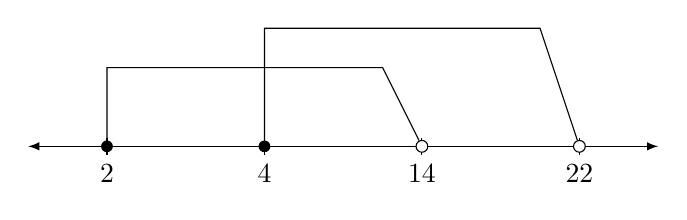
\begin{tikzpicture}
        \draw[latex-latex] (0, 0) -- (8, 0);
        \draw[shift={(1, 0)}, color=black] (0pt, 3pt) -- (0pt, -3pt) node[below] {$2$};
        \draw[shift={(3, 0)}, color=black] (0pt, 3pt) -- (0pt, -3pt) node[below] {$4$};
        \draw[shift={(5, 0)}, color=black] (0pt, 3pt) -- (0pt, -3pt) node[below] {$14$};
        \draw[shift={(7, 0)}, color=black] (0pt, 3pt) -- (0pt, -3pt) node[below] {$22$};
        \node[circle,fill,inner sep=1.5pt](a)at(1,0){};
        \node[circle,fill,inner sep=1.5pt](b)at(3,0){};
        \node[circle,draw,fill=white,inner sep=1.5pt](c)at(5,0){};
        \node[circle,draw,fill=white,inner sep=1.5pt](d)at(7,0){};
        \draw[black] (a) -- (1, 1) -- (4.5, 1) -- (c);
        \draw[black] (b) -- (3, 1.5) -- (6.5, 1.5) -- (d);
    \end{tikzpicture}
\end{center}

\sout{눈금 선형 아닌건 안비밀} \newline

여기에 $A_3$까지 그려보자.

\begin{center}
    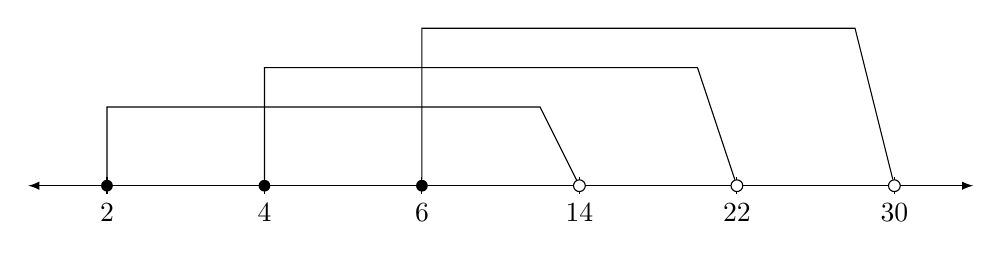
\begin{tikzpicture}
        \draw[latex-latex] (0, 0) -- (12, 0);
        \draw[shift={(1, 0)}, color=black] (0pt, 3pt) -- (0pt, -3pt) node[below] {$2$};
        \draw[shift={(3, 0)}, color=black] (0pt, 3pt) -- (0pt, -3pt) node[below] {$4$};
        \draw[shift={(5, 0)}, color=black] (0pt, 3pt) -- (0pt, -3pt) node[below] {$6$};
        \draw[shift={(7, 0)}, color=black] (0pt, 3pt) -- (0pt, -3pt) node[below] {$14$};
        \draw[shift={(9, 0)}, color=black] (0pt, 3pt) -- (0pt, -3pt) node[below] {$22$};
        \draw[shift={(11, 0)}, color=black] (0pt, 3pt) -- (0pt, -3pt) node[below] {$30$};
        \node[circle,fill,inner sep=1.5pt](a)at(1,0){};
        \node[circle,fill,inner sep=1.5pt](b)at(3,0){};
        \node[circle,fill,inner sep=1.5pt](c)at(5,0){};
        \node[circle,draw,fill=white,inner sep=1.5pt](d)at(7,0){};
        \node[circle,draw,fill=white,inner sep=1.5pt](e)at(9,0){};
        \node[circle,draw,fill=white,inner sep=1.5pt](f)at(11,0){};
        \draw[black] (a) -- (1, 1) -- (6.5, 1) -- (d);
        \draw[black] (b) -- (3, 1.5) -- (8.5, 1.5) -- (e);
        \draw[black] (c) -- (5, 2) -- (10.5, 2) -- (f);
    \end{tikzpicture}
\end{center}

\sout{눈금 스케일 아는분 찾아요} \newline

사실 눈치 빠른 사람이라면 지금쯤 $A_1$부터 $A_n$까지 합집합한 것이 $A_1$과 $A_n$을 합집합한 것과 같다는 것을 알게 되었을 것이다. 따라서 사실

\[
    S = A_1 \cap A_n = \{x \mid 2n \le x < 14\, x \in \mathbb{N}\}
\]

이고, 따라서 $S \not = \varnothing$인 $n$의 최댓값은 6이므로 $a = 6$, 이때 $S = \{12, 13\}$이므로 $b = 2$, $a + b = \underline{8}$이다.

\paragraph{4번}

\subparagraph{보기 ㄱ} $m$과 $n$이 서로소이어도 공통인 약수 1을 가지므로 $A_m \cap A_n \not = \varnothing$이다.

\subparagraph{보기 ㄴ} $k \in A_m$인 모든 $k$에 대해, 자연수 $p$에 대하여 $kp = n$이므로 맞는 보기이다.

\subparagraph{보기 ㄷ} $m$과 $n$의 최대공약수가 $G$이고, $m = aG$, $n = bG$ (단, $a$와 $b$는 서로소)일때 주어진 식을 다음과 같이 쓸 수 있다.

\[
    (A_{aG} \cap A_{bG}) \subset A_{(a + b)G}
\]

$A_{aG} \cap A_{bG}$는 $A_{aG}$와 $A_{bG}$의 공약수의 집합이므로 $A_G$와 같다. 따라서 보기 ㄴ에 의해

\[
    A_{aG} \cap A_{bG} = A_G \subset A_{(a + b)G}
\]

가 성립한다.

\paragraph{5번}
$A$의 모든 원소 합이 28이고, $A \cup B$의 모든 원소 합이 55이므로 다음과 같은 식이 성립한다.

\[
    a_1 + a_2 + a_3 + a_4 + a_5 = 28
\]
\[
    2(a_1 + a_2 + a_3 + a_4 + a_5) + 5d - (4 + 7) = 55
\]

이 식들을 통해 $d = 2$임을 알 수 있고, $A \cap B = \{4, 7\}$이므로 $\{4, 7\} \subset A$이고, $\{4, 7\} \subset B$임을 알 수 있다. 또한, 

\[
B = \{a_i + d \mid a_i \in A\} = \{a_i + 2 \mid a_i \in A\}
\]

이고, 이를 거꾸로 이용하면 $A = \{b_i - d \mid b_i \in B\} = \{b_i - 2 \mid b_i \in B\}$이므로 $\{2, 5\} \subset A$이다. $A$의 모든 원소의 합은 28이므로 $A = \{2, 4, 5, 7, 10\}$이고, 가장 큰 원소와 가장 작은 원소의 곱은 \underline{20}.
\end{document}
